%%%%%%%%%%%%%%%%%%%%%%%%%%%%%%%%%%%%%%%%%%%%%%%%%%%
% DOCUMENT CLASS DECLARATION
%%%%%%%%%%%%%%%%%%%%%%%%%%%%%%%%%%%%%%%%%%%%%%%%%%%
%% Use the following options:
% \documentclass[paper type% ("letterpaper" required)
% , one or two sided% ("oneside" or "twoside")%
% , font size% ("12pt" required)%
% , document type% ("these", "memoire", "memoirepararticles", "memoireprojet" or "thesepararticles")%
% , document language ("francais" or "english)%
% , addition options% ("creativecommons" if the document is under the creative commons license, "hyperref", "withAlgo2e" to use algorithm2e package with proper formating)
%]{thETS}

%% Exemple with a Ph.D thesis under creative commons, using hyperref
\documentclass[letterpaper%
, twoside%
, 12pt%
,thesepararticles%
, english%
,creativecommons,hyperref, withAlgo2e%
]{thETS}

%%%%%%%%%%%%%%%%%%%%%%%%%%%%%%%%%%%%%%%%%%%%%%%%%%%
% IMPORTANT: PRINTING WITH THE PROPER MARGINS
%%%%%%%%%%%%%%%%%%%%%%%%%%%%%%%%%%%%%%%%%%%%%%%%%%%
%% Always set the "scaling" option to "none" in the prining options 
%% to print the generated PDF with the proper margins.
%%%%%%%%%%%%%%%%%%%%%%%%%%%%%%%%%%%%%%%%%%%%%%%%%%%


%%%%%%%%%%%%%%%%%%%%%%%%%%%%%%%%%%%%%%%%%%%%%%%%%%%
% DECLARATION OF AN ADDITION LIST OF REFERENCES
%%%%%%%%%%%%%%%%%%%%%%%%%%%%%%%%%%%%%%%%%%%%%%%%%%%
%% Exemple of an additional list of references called "refs"
% "refs" is used as a suffix to all bibliography related commands
\newcites{refs}{LIST OF REFERENCES}

%%%%%%%%%%%%%%%%%%%%%%%%%%%%%%%%%%%%%%%%%%%%%%%%%%%
% TITLE PAGE OPTIONS
%%%%%%%%%%%%%%%%%%%%%%%%%%%%%%%%%%%%%%%%%%%%%%%%%%%

\title{Adaptive Collaborative  Autonomous Wireless Networks}

\author{Aytac OZKAN}
\authorcopyright{Aytac Ozkan}

\datesoutenance{"Defense date"}

\datedepot{"Deposit Date"}

\directeur{Prof. Dr.}{Kim Khoa Nguyen}{Department of Electrical Engineering and University of Quebec}

%\directeur{Mrs.}{Prénom Nom}{Nom du département et institution}

\codirecteur{M.}{Pr. Louis Rivest}{PhD Program's Director}

%\codirecteurB{M.}{Prénom Nom}{département et institution}

\president{M.}{First Name Last Name}{Department and institution}

\examinexterne{M.}{First Name Last Name}{Department and institution}

%\jury{Mme.}{Prénom Nom}{département et institution}{}

%%%%%%%%%%%%%%%%%%%%%%%%%%%%%%%%%%%%%%%%%%%%%%%%%%%
% CHANGING THE NAME OF THE DIPLOMA
%%%%%%%%%%%%%%%%%%%%%%%%%%%%%%%%%%%%%%%%%%%%%%%%%%%
%% It is possible to change the name of the diploma to append the concentration by defining \concentration
%\newcommand{\concentration}{ELECTRICAL ENGINEERING}

\listfiles

%%%%%%%%%%%%%%%%%%%%%%%%%%%%%%%%%%%%%%%%%%%%%%%%%%%
% ACTUAL DOCUMENT
%%%%%%%%%%%%%%%%%%%%%%%%%%%%%%%%%%%%%%%%%%%%%%%%%%%
\begin{document}

\pagenumbering{Roman}

%%- Title page -%%
\maketitle

%%- Jury presentation -%%
\presentjury

%%- Foreword -%%
\begin{foreword}

\lipsum[1] % Texte de remplissage pour donner un exemple de la mise en page

\end{foreword}



%%- Acknowledgements -%%
\begin{acknowledgements}

\lipsum[1] % Text filling, to have an example of the layout


\end{acknowledgements}


%%- Summary -%%

\begin{summary}{French title}{mot-clé1, mot-clé2}

\lipsum[1] % Text filling, to have an example of the layout

\end{summary}


%%- Abstract -%%
\begin{abstract}{reinforcement-Learning, transfer-learning,wireless-networks,anti-jamming,multi-agent, collaborative-learning}

Due to tremendous improvements of technology, the world is more connected than ever at the human history. Mobile devices, cell phones, smart home solutions, autonomous cars etc. These vehicles are usually using IEEE 802.15.4 communication protocols, the devices which uses this protocol has the limited number of communication channels and low transmit power, are especially susceptible for the jamming attacks. For example, some internet of things (IoT) devices (e.g., brain and heart inculcated IoT devices), jamming attacks can cause serous consequences for human health

Within this concern, to prevent this kind of intentional interference against the wireless networks, we are going to employ self learning algorithms such as deep reinforcement learning to develop resilient, intelligent, and self-supervised anti-jamming framework.

 Since, The DeepMind has been introduced the Reinforcement Learning (RL) and Q-Learning algorithm \cite{ACM:HasseltetSilver}, this tools become one of the major toolkit to develop mitigation and intelligent deceptions strategies to prevent against reactive jamming attacks. Despite it is a subset of machine learning \cite{Kasturi2020MachineLR},it is no need long training times and huge datasets, and this future is the key of its success at the field. 

\end{abstract}


%%- Table of contents -%%
\tableofcontents


%%- List of tables -%%
\listoftables


%%- List of figures -%%
\listoffigures

\listofalgorithms


%%- List of abbreviations -%%
\begin{listofabbr}[3cm]
\item [ETS] École de Technologie Supérieure
\item [ASC] Agence Spatiale Canadienne
\end{listofabbr}


%%- List of symbols -%%
\begin{listofsymbols}[3cm]
\item [a] Première lettre de l'alphabet
\item [A] Première lettre de l'alphabet en majuscule
\end{listofsymbols}


\cleardoublepage

\pagenumbering{arabic}

% Marginpar to the left of the document
\reversemarginpar

%%%%%%%%%%%%%%%%%%%%%%%%%%%%%%%%%%%%%%%%%%%%%%%%%%%
% THESIS EXAMPLE
%%%%%%%%%%%%%%%%%%%%%%%%%%%%%%%%%%%%%%%%%%%%%%%%%%%

\begin{introduction}

The last decade has witnessed the rapid growth of Machine Learning (ML) applications in wireless networks thanks to its agility and efficacy, especially in dealing with uncertainty and dynamics in large-scale problems
    \cite{8743390} \cite{6336689}
However, some recent studies have revealed that conventional ML solutions have shortcomings, especially when they are applied to solve emerging problems in wireless networks, due to special characteristics of wireless communications, such as high mobility, dynamic environments, diverse connections, and interferenceHowever, some recent studies have revealed that conventional ML solutions have shortcomings, especially when they are applied to solve emerging problems in wireless networks, due to special characteristics of wireless communications, such as high mobility, dynamic environments, diverse connections, and interference.

Moreover, the performances of ML techniques mainly rely on the availability of training data, but acquiring a sufficient amount of data might be costly and time-consuming. Even if the training data are sufficient, conventional ML techniques usually require a long training time, which makes them impractical for many latency-sensitive applications. Apart from the training time issues, many wire- less devices, e.g., IoT devices, are constrained by their limited computing capacity, and thus they are unable to run high-complexity ML tasks. Moreover, many ML techniques actually create more wireless traffic demands because data have to be sent to a central node for training and processing. Beside causing higher communication overhead, sending raw data may also threaten network users' privacy because sensitive information, e.g., healthcare, is sent via the wireless networks.

To address these challenges, Transfer Learning (TL) has recently emerged as a highly-effective solution. Unlike conventional ML techniques that are trained to solve a specific problem, TL leverages valuable knowledge from similar tasks and previous experiences to significantly enhance the learning performance of conventional ML techniques

 As a result, TL possesses various advantages over traditional ML approaches which can be summarized as follows;
 
\begin{itemize}
	\item Enhance quality and quantity of training data: One of the most challenging tasks for conventional ML approaches is finding sufficient and high-quality data for the training process. TL can easily overcome this problem by selecting and transferring knowledge from similar domains with a large amount of high-quality data. As a result, TL has been considered to be a highly-effective solution for ML-based wireless networks in the future.
	\item Speed-up learning processes: Instead of learning from scratch like conventional ML approaches, the training process in TL can be significantly sped up thanks to valuable knowledge shared from other similar domains and/or learned in the past. As a result, this can remarkably improve the learning rate, which is especially crucial for the development of ultra-low latency applications for future wireless networks.
	\item Reduce computing demands: Conventional ML approaches usually require a huge amount of computing resources for the training processes. However, with TL, most of the data were trained by other source domains before the trained models are transferred to the target do- main, thereby significantly reducing computing demands for the training process at the target domain. This is particularly useful for wireless devices (e.g., smartphones and edge devices) as they usually have hardware constraints.
	\item Mitigate communication overhead: For TL approaches, instead of sending the raw data with large sizes, only knowledge, e.g., weights of trained models, needs to be sent. As a result, the communication overhead can be significantly reduced for the wireless networks.
	\item{Protect data privacy: In TL, instead of learning from raw data from other domains, ones only need to learn from their trained models (expressed through weights), and thus data privacy can be protected. This feature of TL is very helpful for privacy-sensitive wireless applications such as healthcare and military communication networks.}
\end{itemize}

\end{introduction}

%%- Uncomment the literature review for a thesis by articles -%%
%\begin{literaturereview}

%\end{literaturereview}

%%- First demo chapter -%%
\chapter{Research Objectives, Motivation, Research Questions}

\section{Research Objectives}

The main purpose of this research is develop efficient, reliable and relentless mitigation techniques against the jammer particularly reactive and powerful ones by employing machine learning (ML) and wireless communication technologies. 

To achieve the objective defined above, we are going to use the Frequency Hopping Spectrum  Sensing (FHSS) techniques. In the infinite time space, regarding the probability distribution of incoming signals, we are going to build the most accurate ML model to find out  the optimal and the feasible prediction for communication channels.

Of course, the first paragraph is specified only the core part of communication node, but the particular contribution of this research is to develop multi-agent (multi-node) collaborative (transfer meta-learning) learning techniques to satisfy the constraints such as cost of learning (for each node), cost of transferring mitigation strategy. Predicate on these details, we would like to acquire an augmented Markov decision tuple for our ML model.

So we can divide our main objective into three sub sections and each of them address different research problem, 

We assume in the wireless ad-hoc network, there are two communication node (CN) and one reactive jammer. Also CN1 and CN2 has data connection, which means they can transmit to the data to each other. In addition, the ad-hoc network is multi-channel. Constraints, respectively CN's power storage (limit), channel bandwidth, installed CPU or GPU power on the CN. 

\subsubsection{Objectives}

\begin{itemize}
 \item {In the infinite time space, we are going to build a Machine Learning model which will take as input frequencies by sensing from the wireless network, and try to predict jammer next action (channel estimation), literally means that try to find out the next communication channel will jam. And it will allow us to find out the Jamming activity pattern in the ad-hoc network, and by analyzing these patterns we are going to concrete  mitigation strategies. So, related research will propose novel techniques to answer the question below,
     
     How to catalyze the jamming activity pattern and initialize effective and relentless mitigation strategies for the communication nodes in wireless ad-hoc networks by using autonomous learning techniques ?}
 \item {In the first item, we have proposed a method which allows us to analyze the jammer behaviour pattern, and generate defence strategies for the CN based on this pattern. But in the wireless spectrum we have two different CNs and we can have more nodes, in this case we may transfer the produced policy (or strategy) from one node to another when suitable conditions satisfied. Also collaborative learning can increase to chances to mitigate against reactive and powerful jammer by saving time and energy of CNs. E.g, cost of learning, cost of transmission and accuracy of learning models have  high importance roles in decision model of the framework. 
  
 	So, related research will address the question below, 
 	How the collaborative (transfer) learning can assist knowledge transmission between two different communication nodes in the wireless ad-hoc communication spectrum ? 
 }

 \item{In second item we introduced collective (transfer learning) technique, but when a jamming attack hit the wireless network, there won't be any data transmission in this condition, each CNs have to run their own learning algorithm. } 
 
 \end{itemize}


\subsection{Equations tests}

Layout of the equations:

\begin{equation}
   \beta = 8
\end{equation}

\begin{equation}
   \gamma = \alpha \times 3
\end{equation}

\section{Second section}

Example of a second section, to test the layout in the table of contents.

\begin{algorithm}[!h]

\caption{Algorithm example}

\KwIn{Gallery with initial templates $\mathcal G = \{\textbf{r}_1,...,\textbf{r}_J\}$, unlabeled adaptation set $\mathcal D = \{\textbf{d}_{1},...,\textbf{d}_{L}\}$}
\KwOut{Updated Gallery $\mathcal G' = \{\textbf{r}_1,...,\textbf{r}_{J'}\}$, $J' \geq J$}
\BlankLine
\BlankLine

Estimate updating threshold $\gamma^u \geq \gamma^d$ from $\mathcal G$\;

$\mathcal G \leftarrow \mathcal G'$\tcc*{update gallery}

	\For{all samples $d_l \in \mathcal D$ ($l=1,...,L$)}{
		\For{all references $r_j \in \mathcal G$ ($j=1,...,J$)}{
			$s_j(\textbf{d}_l) \leftarrow similarity\_measure(\textbf{d}_l,\textbf{r}_j)$\;
		}
	}
	
	$S(\textbf{d}_l) \leftarrow \max\limits_{j \in [1,J]}\{s_j(\textbf{d}_l)\}$\;
	
	\If{$S(\textbf{d}_l) \geq \gamma_d$}{
		Output positive prediction\;
		
		\If{$S(\textbf{d}_l)\geq \gamma^u$}{
			$\mathcal{G'} \leftarrow \mathcal{G'} \cup \textbf{d}_l$\;
		}
		
	}
\end{algorithm}

%%- Second demo chapter -%%
\chapter{Literature Review}

\section{Table layout tests}

Tables have the same constraints than the figures, except for the caption that has to be on top.


\begin{table}
\centering
		\parbox{0.65\textwidth}{\caption{Test of a long table caption, with linebreak}} % Contrainte manuelle de la largeur de la légende
		
		\begin{tabular}{|c|c|c|c|c|c|c|c|}
		\hline
			{\bf titre} & {\bf titre} & {\bf titre} & {\bf titre} & {\bf titre} & {\bf titre} & {\bf titre} & {\bf titre} \\
	  \hline
			blá & blá & blá & blá & blá & blá & blá & blá \\
	  \hline
			blá & blá & blá & blá & blá & blá & blá & blá \\
	  \hline
			blá & blá & blá & blá & blá & blá & blá & blá \\
	  \hline
			blá & blá & blá & blá & blá & blá & blá & blá \\
	  \hline
			blá & blá & blá & blá & blá & blá & blá & blá \\
	  \hline
			blá & blá & blá & blá & blá & blá & blá & blá \\
	  \hline
		\end{tabular}
\end{table}


\chapter{Proposed methodologies}
\chapter{Preliminary Results}


%%- Conclusion -%%
\begin{conclusion}

\lipsum[1] % Text filling, to have an example of the layout

\end{conclusion}


%%%%%%%%%%%%%%%%%%%%%%%%%%%%%%%%%%%%%%%%%%%%%%%%%%%
%  Appendix example:
%%%%%%%%%%%%%%%%%%%%%%%%%%%%%%%%%%%%%%%%%%%%%%%%%%%
\appendix

%% To use more than one appendix
\multiannexe

%% Appendix from an external file
% \include{extApp}

\chapter{Appendix example}


\section{First section of the appendix}


\subsection{Figures in annexes}

\begin{figure}
	\centering
	\fbox{
		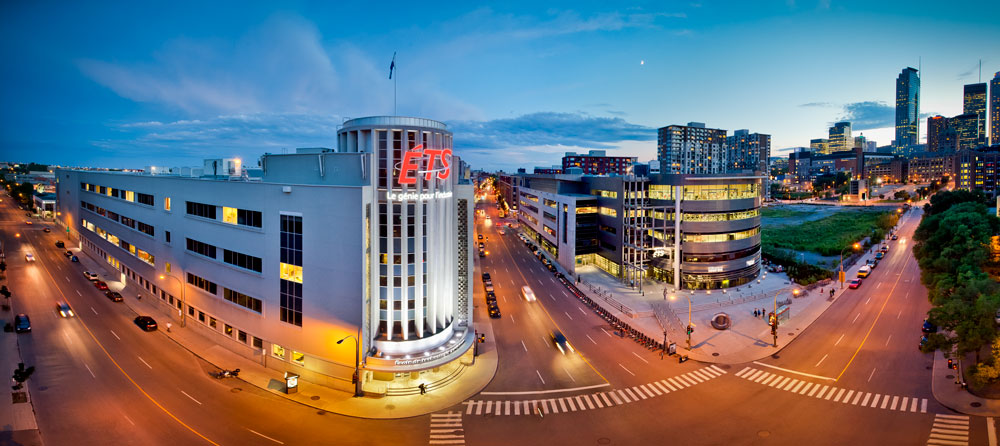
\includegraphics[width=0.75\textwidth]{Figures/vueEts.jpg}
	}
	 \\ \parbox{0.7\textwidth}{\caption{Figure in an appendix}\label{fig:testAp}}
\end{figure}

\begin{figure}
	\centering
	\fbox{
	\parbox{0.975\linewidth}{
	\subfloat[first figure]{
		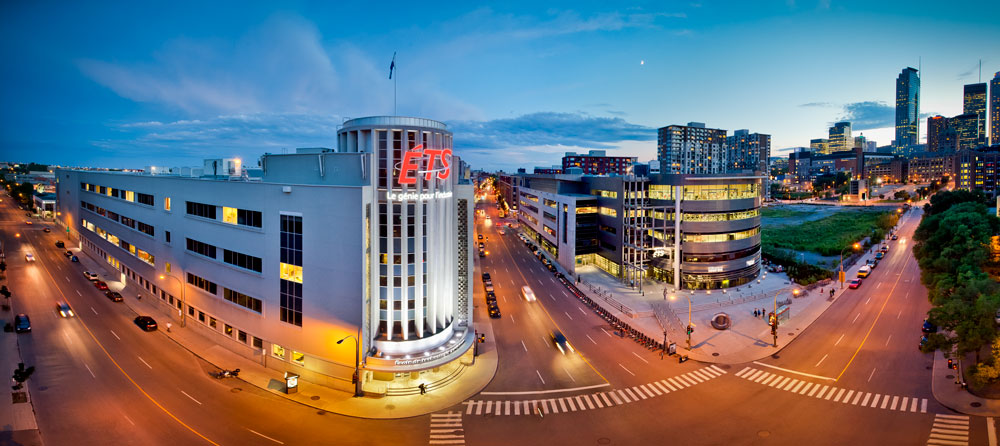
\includegraphics[width=0.47\linewidth]{Figures/vueEts.jpg}
	}\hspace{0.009\linewidth}
	\subfloat[second figure]{
		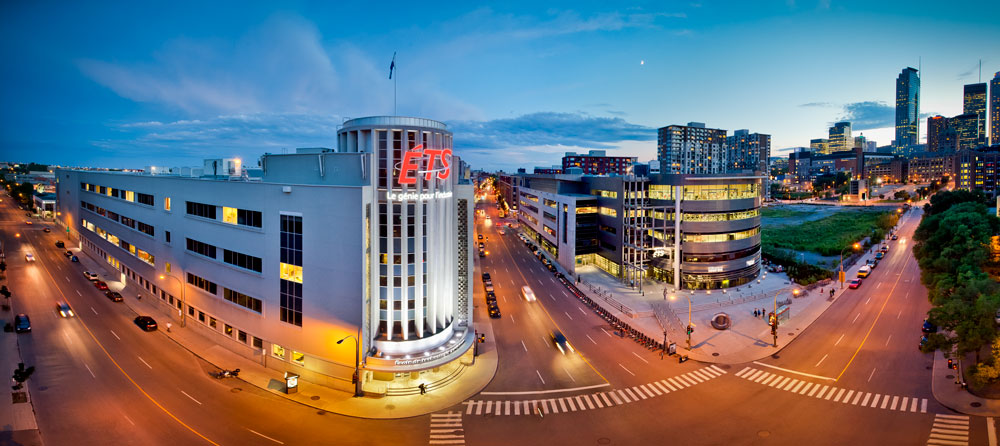
\includegraphics[width=0.47\linewidth]{Figures/vueEts.jpg}
	}
	
	\subfloat[third figure]{
		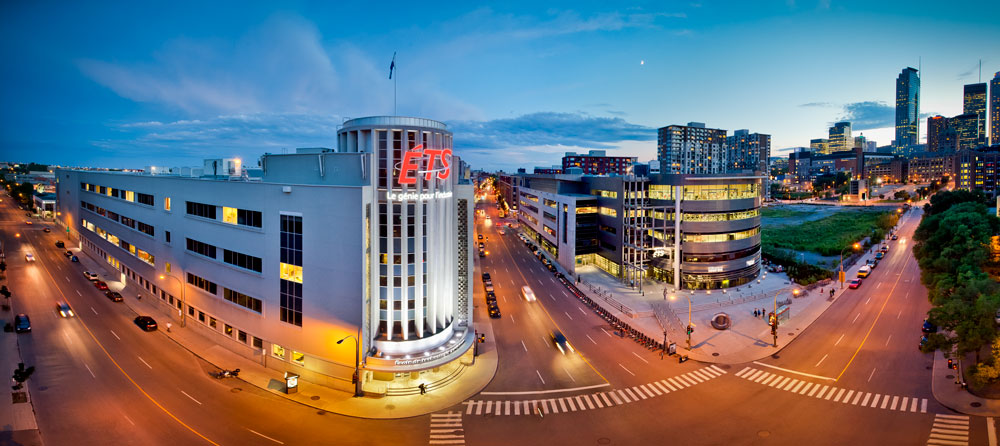
\includegraphics[width=0.47\linewidth]{Figures/vueEts.jpg}
	}\hspace{0.009\linewidth}
	\subfloat[fourth figure]{
		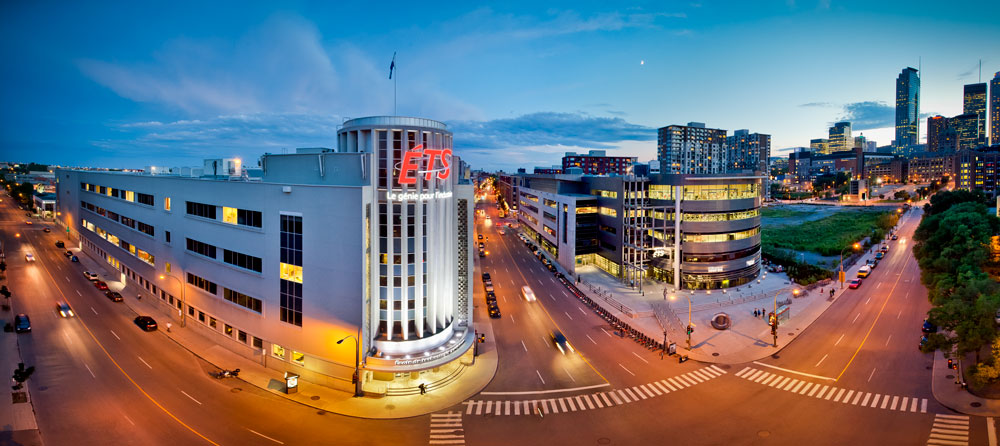
\includegraphics[width=0.47\linewidth]{Figures/vueEts.jpg}
	}}}
	\\ \parbox{0.975\linewidth}{\caption{Subfig example}}
\end{figure}

In the annexes, the figures are declared in the same way. Their numbering changes automatically (e.g. Figure \ref{fig:testAp}).

\subsubsection{Tables in annexes}

\begin{table}
		\parbox{0.65\textwidth}{\caption{Table in an appendix}\label{tab:testAp}}

		\begin{tabular}{|c|c|c|c|c|c|c|c|}
		\hline
			{\bf titre} & {\bf titre} & {\bf titre} & {\bf titre} & {\bf titre} & {\bf titre} & {\bf titre} & {\bf titre} \\
	  \hline
			blá & blá & blá & blá & blá & blá & blá & blá \\
	  \hline
			blá & blá & blá & blá & blá & blá & blá & blá \\
	  \hline
			blá & blá & blá & blá & blá & blá & blá & blá \\
	  \hline
			blá & blá & blá & blá & blá & blá & blá & blá \\
	  \hline
			blá & blá & blá & blá & blá & blá & blá & blá \\
	  \hline
			blá & blá & blá & blá & blá & blá & blá & blá \\
	  \hline
		\end{tabular}
\end{table}

Same behaviour for the tables (e.g., Table \ref{tab:testAp}).


%%%%%%%%%%%%%%%%%%%%%%%%%%%%%%%%%%%%%%%%%%%%%%%%%%%
% BIBLIOGRAPHY AND REFERENCES
%%%%%%%%%%%%%%%%%%%%%%%%%%%%%%%%%%%%%%%%%%%%%%%%%%%

%%- Bibliography -%%
\newpage
% Single spacing for the bibliography
\begin{spacing}{1}
    \setlength{\bibsep}{\baselineskip}
	\nocite{*} % The "nocite" command can be used to print references that haven't been used in the document. The "*" option specifies that every reference should be printed
	\bibliographystyle{bibETS} % ETS bibliography style
	\addcontentsline{toc}{chapter}{BIBLIOGRAPHY} % Addition of the bibliography in the table of contents

	\bibliography{biblio_en} % List of bibliography files, biblio.bib is an example

\end{spacing}

%%- Other list of references, "refs" example --%
%%%%%%%%%%%%%%%%%%%%%%%%%%%%%%%%%%%%%%%%%%%%%%%%%%%
% IMPORTANT: HOW TO COMPILE AND PRINT ADDITIONAL REFERENCES (replace "refs" by the chosen name)
%%%%%%%%%%%%%%%%%%%%%%%%%%%%%%%%%%%%%%%%%%%%%%%%%%%
% Follow these three steps:
%   1. Compile the document once, to save the used references in refs.aux
%   2. Compile the references
% 		- On Linux: Use the "bibtex refs" command in the document folder
%		- On MacOSX (MacTex distribution): Use the "/usr/texbin/bibtex refs" command in the document folder
%		- On Windows: Edit the "update_refs.bat" script to put the right suffix ("refs" here), and launch the script
%   3. Recompile the document TWICE
%%%%%%%%%%%%%%%%%%%%%%%%%%%%%%%%%%%%%%%%%%%%%%%%%%%

\newpage
% Same commands than for the bibliography, only with the "refs" suffix
\begin{spacing}{1}
    \setlength{\bibsep}{\baselineskip}
	%\nociterefs{*}
	\bibliographystylerefs{bibETS}
	\addcontentsline{toc}{chapter}{LIST OF REFERENCES}

	\bibliographyrefs{refs}

\end{spacing}

\end{document}